\documentclass[a4paper,10pt,twocolumn]{article}
\usepackage{amsmath}
\usepackage[english]{babel}
\usepackage[style=ieee,backend=bibtex]{biblatex} \bibliography{ref.bib}
\usepackage{booktabs}
\usepackage[hidelinks]{hyperref}
\usepackage{fancyhdr}
\usepackage{float}
\usepackage{graphicx}
\usepackage[latin1]{inputenc}
\usepackage{nomencl}
\usepackage{mhchem}
\usepackage{multicol}
\usepackage{pgfplots}
    \pgfplotsset{compat=newest} 
    \pgfplotsset{plot coordinates/math parser=false} 
    \newlength\figureheight 
    \newlength\figurewidth 
\usepackage{siunitx}
\usepackage{tikz}
    \usetikzlibrary{arrows}
    \usetikzlibrary{patterns}
    \usetikzlibrary{3d}
    \usetikzlibrary{plotmarks}
\usepackage{tikz-3dplot}
\usepackage{titling}
\usepackage{threeparttable}
\usepackage{xspace}

\newcommand{\Comsol}{\textsc{Comsol}\xspace}
\newcommand{\comsol}{\textsc{comsol}\xspace}
\newcommand{\ComsolMultiphysics}{%
    \textsc{Comsol}~Multiphysics\textsuperscript{\textregistered}\xspace}
\newcommand{\Cmos}{\textsc{Cmos}\xspace}
\newcommand{\cmos}{\textsc{cmos}\xspace}
\newcommand{\Fem}{\textsc{Fem}\xspace}
\newcommand{\fem}{\textsc{fem}\xspace}
\newcommand{\Ic}{\textsc{Ic}\xspace}
\newcommand{\ic}{\textsc{ic}\xspace}
\newcommand{\Mems}{\textsc{Mems}\xspace}
\newcommand{\mems}{\textsc{mems}\xspace}
\newcommand{\Rtd}{\textsc{Rtd}\xspace}
\newcommand{\rtd}{\textsc{rtd}\xspace}

% Top matter
\title{\Mems Multimorph Capacitive Temperature Sensors in \ComsolMultiphysics}
\author{Z0966990}
\date{\today}

% Headers and footers
\pagestyle{fancy}
\fancyhf{}
\lhead{
\includegraphics[width=0.1\textwidth]{img/Durham.png}}
\chead{\thetitle}
\rhead{\theauthor}
\cfoot{\thepage}

\begin{document}

% Title and abstract
\thispagestyle{plain}

\twocolumn[{
\begin{@twocolumnfalse} \centering
    % 
\includegraphics[width=0.2\textwidth]{img/Durham.png}\\
    \Large\thetitle
    \vskip0.2em
    \large Level 3 Semiconductor, Physics and Devices\\
    \vskip0.4em
    \large\theauthor\\
    \vskip0.4em
    \large\thedate\\
    \hrulefill
    \renewcommand{\abstractname}{\large Abstract}
    \begin{abstract}
        This report describes how the $C$--$T$ characteristics of \mems
        multimorph capacitive temperature sensors vary with geometry,     
        material choice and prestress conditions. The sensors were modelled
        using \fem and physics simulation software---\ComsolMultiphysics---so
        the key design parameters, physics modelling choices and mesh analysis
        are also included.
    \end{abstract}
    \vskip\parsep
\end{@twocolumnfalse}
}]


\makenomenclature

% Acronyms
\nomenclature[A0]{\cmos}{Complementary metal oxide semiconductor}
\nomenclature[A1]{\fem}{Finite element modelling}
\nomenclature[A2]{\mems}{Microelectromechanical systems}
\nomenclature[A3]{\rtd}{Resistance temperature detector}

\nomenclature[B0]{$\alpha$}{Thermal expansion coefficient
    \hfill[\si{\per\kelvin}]}

\nomenclature[C0]{$C$}{Capacitance
    \hfill[\si{\farad}]}

\printnomenclature

\section{Introduction}

In an increasingly data centric world, the number of sensors found in
consumer electronics, industrial health monitoring, the automotive industry and
other sectors is expected exceed one trillion in the next 20
years~\cite{bryzek2014emergence}.

\begin{figure}[h]
    \centering
    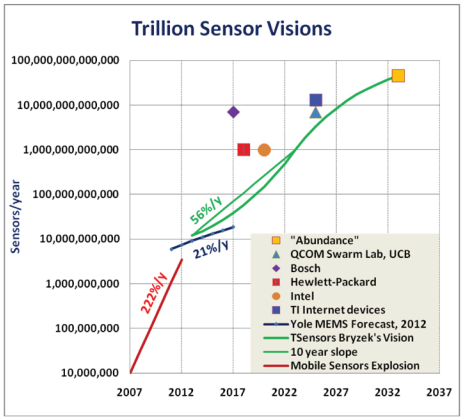
\includegraphics[width=0.4\textwidth]{img/trillion-sensors.png}
    \caption{J. Bryzek's trillion sensor vision~\cite{bryzek2014emergence}.}
    \label{fig:tsensors}
\end{figure}

Temperature sensors make up an sizeable portion of this industry: the demand for
smaller, more efficient and more accurate sensors is rising. There are a few
existing temperature sensors available across different sectors.

\begin{itemize}
    \item Thermistors: which exhibit a non-linear inverted resistive response
    across a wide range of temperatures.
    \item Thermocouples: which generate a non-linear potential difference
    response to across two dissimilar conductors due to a thermoelectric effect.
    \item Resistance thermometers (\rtd{}s): which respond with a very linear
    resistance for some materials: \ce{Pt}, \ce{Cu} and \ce{Ni}.
    \item Silicon bandgap sensors: which respond in conductivity at scales
    suitable for \ic{}s.
\end{itemize}

Multimorph capacitive sensors are an alternative investigated by Scott in his
2012 paper~\cite{scott2012600}. Unlike resistive temperature sensors,
capacitive sensors do not consume power at constant temperature. Low power
consumption combined with small \mems package size means there is opportunity
for these sensors to dominate in portable devices moving forward.

\section{Background}

A multimorph is a cantilever composed of layers of with increasing expansion
coefficients. When current travels in opposite directions through
two piezo-electric multimorphs layers, the layers are subjected to different
stresses and the cantilever deflects. This is an actuator.

Temperature responsive multimorphs are composed of layers with increasing
thermal expansion coefficients. When the multimorph cantilever is heated, it's
temperature increases, the layers expand by differing amounts and the cantilever
deflects. This deflection can be sensed through changing capacitance.

\begin{figure}[h] \centering
    % \includegraphics[width=0.4\textwidth]{img/DEFLECTED-MULTIMORPH.jpg}
    \caption{Cross-section of a temperature sensitive multimorph.}
    \label{fig:multimorph}
\end{figure}

\subsection{Construction}

An effective temperature sensitive multimorph has layers with increasing thermal
expansion coefficients. Scott uses a three layer multimorph with  thermally
grown \ce{SiO2}, vapour deposited \ce{Si3N4}, sputtered \ce{Au}.
Table~\ref{tab:cmos-materials} show the thermal expansion coefficients for a
range of \cmos compatible materials---the majority of those used in \mems
manufacture.

\begin{table}[h]
    \centering
    \begin{threeparttable}
        \caption{Thermal expansion coefficients of some \cmos compatible
        materials~\cite{comsol2017material}.}
        \label{tab:cmos-materials}
        \begin{tabular}{@{}l l S@{}}
            \toprule
            \multicolumn{2}{l}{\cmos compatible material} &
            \multicolumn{1}{r}{$\alpha$~[\si{\per\kelvin}]} \\
            \midrule
            \textbf{Metals} \\
            \hspace{0.5em}Aluminium       & \ce{Al}    & 23.1e-6 \\
            \hspace{0.5em}Gold            & \ce{Au}    & 14.2e-6 \\
            \hspace{0.5em}Titanium        & \ce{Ti}    & 8.6e-6 \\
            \textbf{Semiconductors} \\
            \hspace{0.5em}Silicon         & \ce{Si}    & 2.6e-6 \\
            \textbf{Insulators} \\
            \hspace{0.5em}Silicon Nitrate & \ce{Si3N4} & 2.3e-6 \\
            \hspace{0.5em}Silicon Oxide   & \ce{SiO2}  & 0.5e-6 \\
            \bottomrule
        \end{tabular}
    \end{threeparttable}
\end{table}

By layering \ce{Au} ontop of \ce{Si3N4} ontop of \ce{SiO2} 
(\ce{Au}--\ce{Si3N4}--\ce{SiO2}), Scott was able to design a multimorph 
cantilever with  increasing temperature expansion coefficients and two
boundaries where the  internal stresses of each layer interacted. The cantilever 
to deflected increasingly downwards with temperature.

The \ce{Au} multimorph layer was an easily accessible electrode. However, two
electrodes are required to read the capacitance developed through a flexible
dielectric---air and in this case.  A conductive \ce{Si} substrate acted as a 
fixed electrode on the other side of the air gap, providing mechanical stability 
during operation and fabrication. The oxide layers insulated the moving \ce{Au} 
electrode from the fixed \ce{Si} substrate.

A practical implementation of a multimorph capcitive temperature sensor at least
two layers: a conductive metal contact ontop of one or more insulating oxides.
The cantilever must be mounted ontop of a conductive substrate so the potential
may be measured at both sides of the varying air gap.

\section{Modelling}

The model used and varied in the following experiments was based on the 
\ce{Au}--\ce{Si3N4}--\ce{SiO2} sensor proposed by Scott~\cite{scott2012600}.

\subsection{Geometry}

In \fem computation there is a trade-off between computation time and accuracy,
where computation time and normally accuracy increase with the number of degrees
of freedom. However, techniques can be applied to reduce degrees of freedom
without affecting accuracy. Figure~\ref{fig:model-symmetry} illustrates the
sensor geometry modelled and the lines where the two symmetry planes intersect
external faces.

\begin{figure}[h]
    \centering
    \tdplotsetmaincoords{70}{110}
    \begin{footnotesize}
    \begin{tikzpicture}[scale=0.4\textwidth/0.800cm,tdplot_main_coords]

        % Substrate
        \begin{scope}[canvas is xy plane at z=0.190]
            \path [fill=lightgray!140] (0.000,0.000) -- (0.000,0.840) --
                (0.060,0.840) -- (0.060,0.000) -- (0.000,0.000);
            \draw [thin,dashed] (0.060/2,0.000) -- (0.060/2,0.840);
            \draw (0.060,0.000) -- (0.000,0.000) -- (0.000,0.840);
        \end{scope}
        \begin{scope}[canvas is xy plane at z=0.200]
            \path [fill=lightgray!140] (0.000,0.370) -- (0.000,0.470) --
                (0.060,0.470) -- (0.060,0.370) -- (0.000,0.370);
            \draw [thin,dashed] (0.000,0.840/2) -- (0.060,0.840/2);
            \draw (0.060,0.370) -- (0.000,0.370) -- (0.000,0.470);
        \end{scope}
        \begin{scope}[canvas is zx plane at y=0.470]
            \path [fill=lightgray!120] (0.190,0.000) -- (0.190,0.060) --
                (0.200,0.060) -- (0.200,0.000) -- (0.190,0.000);
            \draw [thin,dashed] (0.190,0.060/2) -- (0.200,0.060/2);
            \draw (0.190,0.000) -- (0.200,0.000);
        \end{scope}
        \begin{scope}[canvas is zx plane at y=0.840]
            \path [fill=lightgray!120] (0.000,0.000) -- (0.000,0.060) --
                (0.190,0.060) -- (0.190,0.000) -- (0.000,0.000);
            \draw [thin,dashed] (0.000,0.060/2) -- (0.190,0.060/2);
            \draw (0.190,0.000) -- (0.000,0.000) -- (0.000,0.060);
        \end{scope}
        \begin{scope}[canvas is yz plane at x=0.060]
            \path [fill=lightgray] (0.000,0.000) -- (0.840,0.000) -- 
                (0.840,0.190) -- (0.470,0.190) -- (0.470,0.200) --
                (0.370,0.200) -- (0.370,0.190) -- (0.000,0.190) --
                (0.000,0.000);
            \draw [thin,dashed] (0.840/2,0.000) -- (0.840/2,0.200);
            \draw (0.370,0.190) -- (0.370,0.200);
            \draw (0.840,0.000) -- (0.000,0.000) -- (0.000,0.190);
        \end{scope}

        % Beam
        \begin{scope}[canvas is xy plane at z=0.209]
            \path [fill=olive!140] (0.020,0.020) -- (0.020,0.820) --
                (0.040,0.820) -- (0.040,0.020) -- (0.020,0.020);
            \draw [thin,dashed] (0.020,0.840/2) -- (0.040,0.840/2);
            \draw [thin,dashed] (0.060/2,0.020) -- (0.060/2,0.820);
            \draw (0.040,0.020) -- (0.020,0.020) -- (0.020,0.820);
        \end{scope}
        \begin{scope}[canvas is zx plane at y=0.820]
            \path [fill=olive!120] (0.206,0.020) -- (0.206,0.040) -- 
                (0.209,0.040) -- (0.209,0.020) -- (0.206,0.020);
            \path [fill=cyan!120] (0.203,0.020) -- (0.203,0.040) -- 
                (0.206,0.040) -- (0.206,0.020) -- (0.203,0.020);
            \path [fill=magenta!120] (0.200,0.020) -- (0.200,0.040) -- 
                (0.203,0.040) -- (0.203,0.020) -- (0.200,0.020);
            \draw [thin,dashed] (0.200,0.060/2) -- (0.209,0.060/2);
            \draw (0.209,0.020) -- (0.200,0.020) -- (0.200,0.040);
        \end{scope}
        \begin{scope}[canvas is yz plane at x=0.040]
            \path [fill=olive] (0.020,0.206) -- (0.020,0.209) -- (0.820,0.209)
                -- (0.820,0.206) -- (0.020,0.206);
            \path [fill=cyan] (0.020,0.203) -- (0.020,0.206) -- (0.820,0.206) --
                (0.820,0.203)-- (0.020,0.203);
            \path [fill=magenta] (0.020,0.200) -- (0.020,0.203) -- (0.820,0.203)
                -- (0.820,0.200)-- (0.020,0.200);
            \draw [thin,dashed] (0.840/2,0.200) -- (0.840/2,0.209);
            \draw (0.820,0.200) -- (0.470,0.200);
            \draw (0.370,0.200) -- (0.020,0.200) -- (0.020,0.209);
        \end{scope}

        % Scale
        \draw [-serif cm] (0.200,0,0) -- ++(-0.050,0,0);
        \draw [-serif cm] (0.200,0,0) -- ++(0,0.050,0) 
            node[right]{\SI{50}{\micro\meter}};
        \draw [-serif cm] (0.200,0,0) -- ++(0,0,0.050);
    \end{tikzpicture}
    \end{footnotesize}
    \caption{Symmetry lines of the multimorph capacitive temperature
    sensor---marked with dashed lines.}
    \label{fig:model-symmetry}
\end{figure}

Rather than mesh the entire geometry, only one of the four symmetric quadrants
was modelled, with symmetric boundary conditions applied to those intersecting
the symmetry planes. The total capacitance of the four parallel quadrants was
then found by multiplying all evaluated readings by four as 
in~\eqref{eq:C-parallel}.
\begin{equation} \label{eq:C-parallel}
    C_{||} = \sum_{i}^4{C_i} = 4C
\end{equation}


Figure~\ref{fig:model-cross-section} details the dimensions and geometric
parameters of the \comsol model.

\begin{figure}[h]
    \centering
    \begin{footnotesize}
    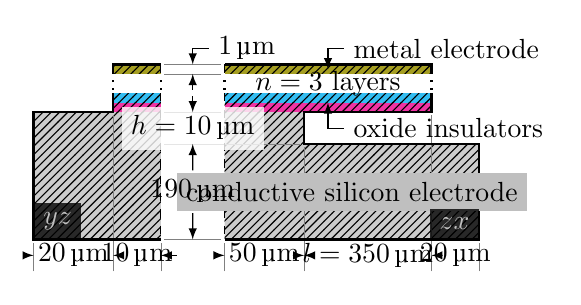
\begin{tikzpicture}[scale=0.4\textwidth/1.2cm]
        % Layers
        \path [fill=olive!80]   (0.20,0.72) rectangle (0.85,0.75);
        \path [fill=cyan!80]    (0.20,0.63) rectangle (0.85,0.66);
        \path [fill=magenta!80] (0.20,0.60) rectangle (0.85,0.63);
        \path [fill=lightgray!80] (0.20,0.20) -- (1.00,0.20) -- (1.00,0.50) -- 
            (0.45,0.50) -- (0.45,0.60) -- (0.20,0.60) -- (0.20,0.20);
        \path [pattern=north east lines] (0.20,0.72) rectangle (0.85,0.75);
        \path [pattern=north east lines] (0.20,0.63) rectangle (0.85,0.66);
        \path [pattern=north east lines] (0.20,0.60) rectangle (0.85,0.63);
        \path [pattern=north east lines] (0.20,0.20) -- (1.00,0.20) --  
            (1.00,0.50) -- (0.45,0.50) -- (0.45,0.60) -- (0.20,0.60) --
            (0.20,0.20);

        \path [fill=olive!80]   (-0.15,0.72) rectangle (0.00,0.75);
        \path [fill=cyan!80]    (-0.15,0.63) rectangle (0.00,0.66);
        \path [fill=magenta!80] (-0.15,0.60) rectangle (0.00,0.63);
        \path [fill=lightgray!80] (-0.40,0.20) rectangle (0.00,0.60);
        \path [pattern=north east lines] (-0.15,0.72) rectangle (0.00,0.75);
        \path [pattern=north east lines] (-0.15,0.63) rectangle (0.00,0.66);
        \path [pattern=north east lines] (-0.15,0.60) rectangle (0.00,0.63);
        \path [pattern=north east lines] (-0.40,0.20) rectangle (0.00,0.60);
        
        % Witness lines
        \draw [gray,ultra thin] (0.01,0.75) -- (0.19,0.75);
        \draw [gray,ultra thin] (0.01,0.72) -- (0.19,0.72);
        \draw [gray,ultra thin] (0.01,0.60) -- (0.19,0.60);
        \draw [gray,ultra thin] (0.01,0.50) -- (0.44,0.50);
        \draw [gray,ultra thin] (0.01,0.20) -- (0.19,0.20);

        \draw [gray,ultra thin] (-0.40,0.10) -- (-0.40,0.19);
        \draw [gray,ultra thin] (-0.15,0.10) -- (-0.15,0.59);
        \draw [gray,ultra thin] (0.00,0.10) -- (0.00,0.19);
        \draw [gray,ultra thin] (0.20,0.10) -- (0.20,0.19);
        \draw [gray,ultra thin] (0.45,0.10) -- (0.45,0.49);
        \draw [gray,ultra thin] (0.85,0.10) -- (0.85,0.59);
        \draw [gray,ultra thin] (1.00,0.10) -- (1.00,0.19);

        % Outline
        \draw [thick] (0.20,0.20) -- (1.00,0.20) -- (1.00,0.50) -- (0.45,0.50)
            -- (0.45,0.60) -- (0.85,0.60) -- (0.85,0.66);
        \draw [dotted,thick] (0.85,0.67) -- (0.85,0.71);
        \draw [thick] (0.85,0.72) -- (0.85,0.75) -- (0.20,0.75);
        \draw [dashed] (0.20,0.75) -- (0.20,0.72);
        \draw [dotted,thick] (0.20,0.67) -- (0.20,0.71);
        \draw [dashed] (0.20,0.66) -- (0.20,0.20);

        \draw [thick] (0.00,0.20) -- (-0.40,0.20) -- (-0.40,0.60) -- 
            (-0.15,0.60) -- (-0.15,0.66);
        \draw [dotted,thick] (-0.15,0.67) -- (-0.15,0.71);
        \draw [thick] (-0.15,0.72) -- (-0.15,0.75) -- (0.00,0.75);
        \draw [dashed] (0.00,0.75) -- (0.00,0.72);
        \draw [dotted,thick] (0.00,0.67) -- (0.00,0.71);
        \draw [dashed] (0.00,0.66) -- (0.00,0.20);

        % Labels
        \node [right] at (0.575,0.80) {metal electrode};
        \draw [latex-] (0.525,0.735) -- (0.525,0.80) -- (0.575,0.80);
        \node at (0.525,0.69) {$n=3$ layers};
        \draw [latex-] (0.525,0.630) -- (0.525,0.55) -- (0.575,0.55);
        \node [right] at (0.575,0.55) {oxide insulators};
        \node [align=center,fill=lightgray] at (0.60,0.35)
            {conductive silicon electrode};
        \node [above right,fill=black,text=lightgray,
            fill opacity=0.8,text opacity=1] at (-0.40,0.20) {$yz$};
        \node [above left,fill=black,text=lightgray,
            fill opacity=0.8,text opacity=1] at (1.00,0.20) {$zx$};


        % Dimensions
        \node [right] at (0.15,0.80) {\SI{1}{\micro\meter}};
        \draw [latex-] (0.10,0.75) -- (0.10,0.80) -- (0.15,0.80);
        \node [fill=white,fill opacity=0.8,text opacity=1] at (0.10,0.55) 
            {$h=\SI{10}{\micro\meter}$};
        \draw [-latex] (0.10,0.67) -- (0.10,0.72);
        \draw [latex-] (0.10,0.60) -- (0.10,0.65);
        \node (d1) at (0.10,0.35) {\SI{190}{\micro\meter}};
        \draw [-latex] [above] (d1) -- (0.10,0.50);
        \draw [-latex] [below] (d1) -- (0.10,0.20);

        \node (d2) at (0.325,0.15) {\SI{50}{\micro\meter}};
        \draw [-latex] [left] (d2)-- (0.20,0.15);
        \draw [-latex] [right] (d2) -- (0.45,0.15);
        \node (d3) at (0.65,0.15) {$l=\SI{350}{\micro\meter}$};
        \draw [-latex] [left] (d3) -- (0.45,0.15);
        \draw [-latex] [right] (d3) -- (0.85,0.15);
        \node at (0.925,0.15) {\SI{20}{\micro\meter}};

        \node at (-0.075,0.15) {\SI{10}{\micro\meter}};
        \draw [latex-] (0.00,0.15) -- (0.05,0.15);
        \node (d4) at (-0.275,0.15) {\SI{20}{\micro\meter}};
        \draw [-latex] [left] (d4)-- (-0.40,0.15);
        \draw [-latex] [right] (d4) -- (-0.15,0.15);


    \end{tikzpicture}
    \end{footnotesize}
    \caption{Cross-section of the multimorph temperature sensor---not to scale.}
    \label{fig:model-cross-section}
\end{figure}

The model was designed with a thick wafer to provide significant stability. In
reality silicon wafers range from \SIrange{200}{300}{\milli\meter}. Here the
substrate was \SI{200}{\micro\meter} thick prior to removing material for the
air gap. An air gap was left in the model so the electric potential could be meshed and simulated.

The sensor was modelled with a margin of \SI{20}{\micro\meter} to determine the 

\subsection{Mesh}

The cuboid nature of the model called for a mapped swept mesh with the greatest
mesh density in cantilever and air gap.

\subsection{Material}
\subsection{Physics}

\section{Results}

\subsection{C--T study}

\subsection{Material study}

\begin{figure}[h]
    \begin{footnotesize}
        % This file was created by matlab2tikz.
%
%The latest updates can be retrieved from
%  http://www.mathworks.com/matlabcentral/fileexchange/22022-matlab2tikz-matlab2tikz
%where you can also make suggestions and rate matlab2tikz.
%
\definecolor{mycolor1}{rgb}{0.00000,0.44700,0.74100}%
\definecolor{mycolor2}{rgb}{0.85000,0.32500,0.09800}%
\definecolor{mycolor3}{rgb}{0.92900,0.69400,0.12500}%
%
\begin{tikzpicture}

\begin{axis}[%
width=0.3\textwidth,
height=0.194\textwidth,
at={(0\textwidth,0\textwidth)},
scale only axis,
unbounded coords=jump,
xmin=0,
xmax=60,
xlabel style={font=\color{white!15!black}},
xlabel={Temperature \si{\celsius}},
ymin=12,
ymax=30,
ylabel style={font=\color{white!15!black}},
ylabel={Capacitance \si{\femto\farad}},
axis background/.style={fill=white},
axis x line*=bottom,
axis y line*=left,
legend style={at={(0.5,1.03)}, anchor=south, legend cell align=left, align=left, draw=white!15!black}
]
\addplot [color=mycolor1, mark=+, mark options={solid, mycolor1}]
  table[row sep=crcr]{%
0	13.6648410785309\\
5	14.4916759166439\\
10	15.5094086786335\\
15	16.8010096767092\\
20	18.49484463766\\
25	20.7771969014692\\
30	24.2820540497028\\
35	nan\\
40	nan\\
45	nan\\
50	nan\\
55	nan\\
60	nan\\
65	nan\\
70	nan\\
75	nan\\
80	nan\\
85	nan\\
90	nan\\
95	nan\\
100	nan\\
};
\addlegendentry{\ce{Al}\tiny($\alpha=\SI{2.31e-05}{\per\kelvin}$)}

\addplot [color=mycolor2, mark=o, mark options={solid, mycolor2}]
  table[row sep=crcr]{%
0	14.9688346633668\\
5	15.6501712728014\\
10	16.4436546810981\\
15	17.3805417263902\\
20	18.4961552351542\\
25	19.8364647423071\\
30	21.4934762266047\\
35	23.7269495667882\\
40	27.312717625232\\
45	nan\\
50	nan\\
55	nan\\
60	nan\\
65	nan\\
70	nan\\
75	nan\\
80	nan\\
85	nan\\
90	nan\\
95	nan\\
100	nan\\
};
\addlegendentry{\ce{Au}\tiny($\alpha=\SI{1.42e-05}{\per\kelvin}$)}

\addplot [color=mycolor3, mark=triangle, mark options={solid, mycolor3}]
  table[row sep=crcr]{%
0	16.0599156302442\\
5	16.5759929951726\\
10	17.147880510609\\
15	17.784319054519\\
20	18.4947045093175\\
25	19.2895668100914\\
30	20.1845120824866\\
35	21.2103974362495\\
40	22.4261166213369\\
45	23.9383182932526\\
50	25.9636690484724\\
55	29.0577968703444\\
60	nan\\
65	nan\\
70	nan\\
75	nan\\
80	nan\\
85	nan\\
90	nan\\
95	nan\\
100	nan\\
};
\addlegendentry{\ce{Ti}\tiny($\alpha=\SI{8.6e-06}{\per\kelvin}$)}

\end{axis}
\end{tikzpicture}%
    \end{footnotesize}
    \caption{}
    \label{fig:material_study.C-T}
\end{figure}

\begin{figure}[h]
    \begin{footnotesize}
        % This file was created by matlab2tikz.
%
%The latest updates can be retrieved from
%  http://www.mathworks.com/matlabcentral/fileexchange/22022-matlab2tikz-matlab2tikz
%where you can also make suggestions and rate matlab2tikz.
%
\definecolor{mycolor1}{rgb}{0.00000,0.44700,0.74100}%
\definecolor{mycolor2}{rgb}{0.85000,0.32500,0.09800}%
\definecolor{mycolor3}{rgb}{0.92900,0.69400,0.12500}%
%
\begin{tikzpicture}

\begin{axis}[%
width=0.4\textwidth,
height=0.258\textwidth,
at={(0\textwidth,0\textwidth)},
scale only axis,
unbounded coords=jump,
xmin=-10,
xmax=15,
xlabel style={font=\color{white!15!black}},
xlabel={Displacement \si{\micro\meter}},
ymin=12,
ymax=30,
ylabel style={font=\color{white!15!black}},
ylabel={Capacitance \si{\femto\farad}},
axis background/.style={fill=white},
axis x line*=bottom,
axis y line*=left,
legend style={at={(0.5,1.03)}, anchor=south, legend cell align=left, align=left, draw=white!15!black}
]
\addplot [color=mycolor1, mark=+, mark options={solid, mycolor1}]
  table[row sep=crcr]{%
12.1772830460825	13.6648410785309\\
9.13869755826485	14.4916759166439\\
6.09313402425773	15.5094086786335\\
3.04620033004022	16.8010096767092\\
-0.0016606872621599	18.49484463766\\
-3.05010675495152	20.7771969014692\\
-6.09949477232682	24.2820540497028\\
nan	nan\\
nan	nan\\
nan	nan\\
nan	nan\\
nan	nan\\
nan	nan\\
nan	nan\\
nan	nan\\
nan	nan\\
nan	nan\\
nan	nan\\
nan	nan\\
nan	nan\\
nan	nan\\
};
\addlegendentry{\ce{Al}\tiny($\alpha=\SI{2.31e-05}{\per\kelvin}$)}

\addplot [color=mycolor2, mark=o, mark options={solid, mycolor2}]
  table[row sep=crcr]{%
7.61437295767633	14.9688346633668\\
5.71264870995948	15.6501712728014\\
3.80834090012571	16.4436546810981\\
1.9015454140768	17.3805417263902\\
-0.00339751868487469	18.4961552351542\\
-1.90851902814607	19.8364647423071\\
-3.81384281695528	21.4934762266047\\
-5.71963254680427	23.7269495667882\\
-7.62575267443897	27.312717625232\\
nan	nan\\
nan	nan\\
nan	nan\\
nan	nan\\
nan	nan\\
nan	nan\\
nan	nan\\
nan	nan\\
nan	nan\\
nan	nan\\
nan	nan\\
nan	nan\\
};
\addlegendentry{\ce{Au}\tiny($\alpha=\SI{1.42e-05}{\per\kelvin}$)}

\addplot [color=mycolor3, mark=triangle, mark options={solid, mycolor3}]
  table[row sep=crcr]{%
4.68789495804691	16.0599156302442\\
3.51570518940953	16.5759929951726\\
2.34339624927957	17.147880510609\\
1.17099532021015	17.784319054519\\
-0.00147412376511847	18.4947045093175\\
-1.17399206557994	19.2895668100914\\
-2.346547304482	20.1845120824866\\
-3.51915446076559	21.2103974362495\\
-4.69189656325893	22.4261166213369\\
-5.86472870118141	23.9383182932526\\
-7.03755713992866	25.9636690484724\\
-8.2109362012596	29.0577968703444\\
nan	nan\\
nan	nan\\
nan	nan\\
nan	nan\\
nan	nan\\
nan	nan\\
nan	nan\\
nan	nan\\
nan	nan\\
};
\addlegendentry{\ce{Ti}\tiny($\alpha=\SI{8.6e-06}{\per\kelvin}$)}

\end{axis}
\end{tikzpicture}%
    \end{footnotesize}
    \caption{}
    \label{fig:material_study.C-T}
\end{figure}

\section{Analysis}
\section{Conclusion}

% \printbibliography

\end{document}